\section{Results}
\label{sec:results}

Every table in this section is a geometric mean of ratios against JSON on
the same case unless it says otherwise; below 1 is smaller or faster than
JSON. The \emph{cases} column is the number of cases the format has a
result for.

\FloatBarrier
\subsection{Size}
\label{sec:size}

\begin{table}[t]
\centering\small
\resulttable{sizes-web}
\caption{Web regime: message size against JSON's, as written (\emph{raw})
and under each compressor, both sides compressed alike. $\dagger$: cases
where the format writes zero bytes are left out of the mean.}
\label{tab:sizes-web}
\end{table}

\begin{table}[t]
\centering\small
\resulttable{sizes-bulk}
\caption{Bulk regime: message size against JSON's.}
\label{tab:sizes-bulk}
\end{table}

\paragraph{Web regime (Table~\ref{tab:sizes-web}).} As written, a \colbin{}
message is \result{size.web.colbin.raw} of the JSON's size, against
\result{size.web.protobuf.raw} for Protocol Buffers,
\result{size.web.msgpack.raw} for MessagePack and \result{size.web.avro.raw}
for Avro. Compression narrows every gap, because a general-purpose
compressor removes much of the redundancy a binary format removes by
construction: under brotli 5 the same four are \result{size.web.colbin.br5},
\result{size.web.protobuf.br5}, \result{size.web.msgpack.br5} and
\result{size.web.avro.br5}. The schemaless formats, and the zero-copy ones,
are within a few percent of compressed JSON: once a server compresses its
responses, they save almost nothing on the wire.
\recheck{the three sentences above describe run1; confirm direction for the
schemaless and zero-copy formats}

\paragraph{Bulk regime (Table~\ref{tab:sizes-bulk}).} With more rows per
table the column layout has more to work with: \colbin{} is
\result{size.bulk.colbin.raw} of JSON as written and
\result{size.bulk.colbin.br5} under brotli 5, where the row formats stay
close to compressed JSON (\result{size.bulk.protobuf.br5} for Protocol
Buffers, \result{size.bulk.avro.br5} for Avro) and Arrow, columnar but
uncompressed, is at \result{size.bulk.arrow.br5}. The column transforms and
the general-purpose compressor are complementary rather than redundant:
delta and frame of reference expose regularities across rows that a
byte-oriented compressor with a bounded window does not find in a row
layout. \recheck{complementarity claim: holds if colbin's br5 ratio is well
below the row formats'}

\begin{table}[t]
\centering\footnotesize
\resulttable{sizes-datasets-web}
\caption{Web regime by dataset: size against JSON's, as written and under
brotli 5.}
\label{tab:sizes-datasets-web}
\end{table}

\paragraph{By dataset (Table~\ref{tab:sizes-datasets-web}).} The mean over
the web regime hides how different its datasets are. On the tabular datasets
\colbin{} is at \result{size.web.tpcds.colbin.br5} (TPC-DS) and
\result{size.web.publicbi.colbin.br5} (Public BI) of brotli-compressed JSON.
On SchemaStore's typed documents, which are small and hold no table, it is
at \result{size.web.schemastore.colbin.br5}, beside
\result{size.web.schemastore.protobuf.br5} for Protocol Buffers and
\result{size.web.schemastore.avro.br5} for Avro: here the three schema-driven
formats do the same thing, and the result is a tie decided by a few bytes
per message. On the dynamic path, where \colbin{} writes field names like
any schemaless format, it is at \result{size.web.schemastore-dynamic.colbin.br5}.
Arrow on SchemaStore shows the fixed cost of a format made for large tables
on a message of a few hundred bytes. The bulk regime by dataset is in the
artifact (\code{tables/sizes-datasets-bulk.tex}).
\recheck{``tie'' on SchemaStore typed; which of colbin / avro is ahead}

\begin{figure}[t]
\centering
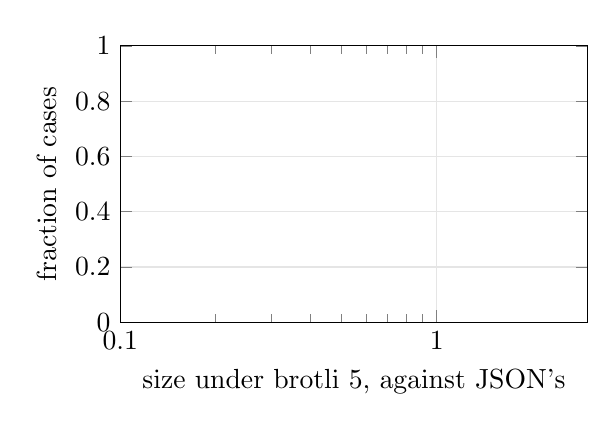
\begin{tikzpicture}
\begin{axis}[width=0.62\linewidth, height=0.42\linewidth,
  xlabel={size under brotli 5, against JSON's}, ylabel={fraction of cases},
  xmode=log, log ticks with fixed point, xmin=0.1, xmax=3, ymin=0, ymax=1,
  legend pos=outer north east, legend style={font=\footnotesize, draw=none},
  cycle list name=color list, grid=major, grid style={gray!20}]
\distcurve{very thick, black}{fig-dist-web-br5-colbin}{colbin}
\distcurve{thick, blue}{fig-dist-web-br5-protobuf}{protobuf}
\distcurve{thick, red}{fig-dist-web-br5-avro}{avro}
\distcurve{thick, orange}{fig-dist-web-br5-msgpack}{msgpack}
\distcurve{thick, teal}{fig-dist-web-br5-arrow}{arrow}
\distcurve{thick, gray}{fig-dist-web-br5-flatbuffers}{flatbuffers}
\end{axis}
\end{tikzpicture}
\caption{Web regime: the distribution over cases of each format's size under
brotli 5 against JSON's under brotli 5. A curve to the left is smaller; each
format's curve is over the cases it carries.}
\label{fig:dist-size}
\end{figure}

Figure~\ref{fig:dist-size} shows the distribution behind the means. The
cases where a format's compressed size exceeds compressed JSON's are the
right-hand tail above 1; for \colbin{} they are small documents, in which
the message is tens of bytes and a compressor's framing dominates.
\recheck{which cases form colbin's tail above 1}

\FloatBarrier
\subsection{Time}
\label{sec:time}

\begin{table}[t]
\centering\small
\resulttable{times-web}
\caption{Web regime: time against JSON's for the same operation
(\result{time.web.cases} cases; access against JSON's decode-fresh, on the
\result{time.web.access.cases} cases that have an access aggregate).}
\label{tab:times-web}
\end{table}

\begin{table}[t]
\centering\small
\resulttable{times-bulk}
\caption{Bulk regime: time against JSON's for the same operation
(\result{time.bulk.cases} cases).}
\label{tab:times-bulk}
\end{table}

\paragraph{Web regime (Table~\ref{tab:times-web}).} \colbin{} encodes in
\result{time.web.colbin.encode} of JSON's time and decodes into a fresh
value in \result{time.web.colbin.decode-fresh}. The formats with generated
code are the ones to compare with: \fmt{vtprotobuf} is at
\result{time.web.vtprotobuf.encode} and
\result{time.web.vtprotobuf.decode-fresh}, generated MessagePack at
\result{time.web.msgpack.encode} and \result{time.web.msgpack.decode-fresh}.
The reflection-based implementations of the same two formats
(\fmt{protobuf}, \fmt{msgpack-reflect}) are several times slower than their
generated counterparts, which is the cost \colbin{}, which generates nothing,
has to avoid by other means: a plan built once per type and executed over
raw pointers. Decoding into a held value is faster than into a fresh one for
every format that can reuse allocations
(\result{time.web.colbin.decode-reuse} for \colbin{}).
\recheck{colbin vs generated code on encode: slower, equal or faster}

\paragraph{Bulk regime (Table~\ref{tab:times-bulk}).} On large tables
\colbin{} encodes in \result{time.bulk.colbin.encode} of JSON's time and
decodes in \result{time.bulk.colbin.decode-fresh}, against
\result{time.bulk.vtprotobuf.encode} and
\result{time.bulk.vtprotobuf.decode-fresh} for \fmt{vtprotobuf} and
\result{time.bulk.arrow.encode} and \result{time.bulk.arrow.decode-fresh}
for Arrow. Decoding a column is a tight loop over one type, where decoding
rows dispatches on a tag per field; and a smaller message is less memory to
read. \recheck{explanation assumes colbin decodes fastest in bulk}

\paragraph{Access without decoding.} The access column is where the
zero-copy formats are in a class of their own: summing one column in place
costs FlatBuffers \result{time.web.flatbuffers.access} and Arrow
\result{time.web.arrow.access} of a JSON decode in the web regime, and Arrow
\result{time.bulk.arrow.access} in the bulk regime, where the column is a
contiguous array. \colbin{} has no access path that avoids decoding: its
\result{time.web.colbin.access} and \result{time.bulk.colbin.access} are a
full decode followed by the sum. An application that reads one field of a
large message and discards the rest is better served by those formats.

\begin{figure}[t]
\centering
\begin{tikzpicture}
\begin{axis}[width=0.48\linewidth, height=0.44\linewidth, title={web},
  xlabel={size under brotli 5}, ylabel={decode-fresh time},
  xmode=log, ymode=log, log ticks with fixed point,
  nodes near coords, point meta=explicit symbolic,
  every node near coord/.append style={font=\tiny, anchor=west},
  grid=major, grid style={gray!20}, enlarge x limits=0.25]
\IfFileExists{\tables/fig-tradeoff-web.dat}{
  \addplot[only marks, mark=*, mark size=1.5pt] table[x=br5, y=decode, meta=format]{\tables/fig-tradeoff-web.dat};}{}
\end{axis}
\end{tikzpicture}\hfill
\begin{tikzpicture}
\begin{axis}[width=0.48\linewidth, height=0.44\linewidth, title={bulk},
  xlabel={size under brotli 5},
  xmode=log, ymode=log, log ticks with fixed point,
  nodes near coords, point meta=explicit symbolic,
  every node near coord/.append style={font=\tiny, anchor=west},
  grid=major, grid style={gray!20}, enlarge x limits=0.25]
\IfFileExists{\tables/fig-tradeoff-bulk.dat}{
  \addplot[only marks, mark=*, mark size=1.5pt] table[x=br5, y=decode, meta=format]{\tables/fig-tradeoff-bulk.dat};}{}
\end{axis}
\end{tikzpicture}
\caption{Size against decode time, both against JSON's, per format and
regime (geometric means; each format over the cases it carries). Down and to
the left is better on both.}
\label{fig:tradeoff}
\end{figure}

\FloatBarrier
\subsection{\colbin{} against each format on common cases}
\label{sec:versus}

\begin{table}[t]
\centering\footnotesize
\resulttable{versus-web}
\caption{Web regime: \colbin{}'s number over each other format's, as a
geometric mean over the cases both carry, and in small type the number of
those cases in which \colbin{}'s is strictly lower. Below 1, \colbin{} is
smaller or faster.}
\label{tab:versus-web}
\end{table}

\begin{table}[t]
\centering\footnotesize
\resulttable{versus-bulk}
\caption{Bulk regime: \colbin{} against each other format on common cases.}
\label{tab:versus-bulk}
\end{table}

The tables above give each format a mean over its own cases.
Tables~\ref{tab:versus-web} and~\ref{tab:versus-bulk} remove that
difference: each row compares \colbin{} with one format on exactly the cases
both carry, and counts the cases \colbin{} wins outright. In the web regime
\colbin{} is smaller than Protocol Buffers under brotli 5 in
\result{vs.web.protobuf.br5.wins} of \result{vs.web.protobuf.br5.n} cases
(mean ratio \result{vs.web.protobuf.br5}) and smaller than Avro in
\result{vs.web.avro.br5.wins} of \result{vs.web.avro.br5.n}
(\result{vs.web.avro.br5}). It encodes faster than \fmt{vtprotobuf} in
\result{vs.web.vtprotobuf.encode.wins} of
\result{vs.web.vtprotobuf.encode.n} cases and faster than generated
MessagePack in \result{vs.web.msgpack.encode.wins} of
\result{vs.web.msgpack.encode.n}, and decodes faster than each in
\result{vs.web.vtprotobuf.decode-fresh.wins} and
\result{vs.web.msgpack.decode-fresh.wins} cases. The rows for \colbin{}'s
own variants measure its options: field tags against none, \fmt{packed5},
and the embedded schema section.

\FloatBarrier
\subsection{What a message is made of}
\label{sec:composition}

\begin{table}[t]
\centering\footnotesize
\resulttable{composition}
\caption{\colbin{} messages by regime and dataset: struct rows at any depth,
the share of them written as table rows, the share of the message's bytes
that are tables, and the schema section (median bytes per case; median
share of the message it describes; the section is not part of the message
unless embedded). The last column is the median of bytes per leaf value.}
\label{tab:composition}
\end{table}

Table~\ref{tab:composition} shows how much of each dataset the table layout
reaches. The tabular datasets are tables almost entirely, by construction.
SchemaStore's documents hold \result{composition.web.schemastore.rows}
struct rows in total, \result{composition.web.schemastore.table-rows}\,\% of
them in tables: on that dataset \colbin{} is a row format, and its results
there measure the row format alone.

The schema section, when embedded, costs its size once per message: a
median of \result{composition.web.publicbi.schema-bytes} bytes on Public BI,
\result{composition.web.publicbi.schema-share}\,\% of the message, and
\result{composition.web.schemastore.schema-bytes} bytes on SchemaStore's
typed documents, where it is \result{composition.web.schemastore.schema-share}\,\%
of a message that is itself tens of bytes. A self-describing message is
nearly free for a table and more than doubles a small document, which is
why a stream of small messages should send the section once per connection
instead. \recheck{``more than doubles'' needs the SchemaStore share above 100}

\FloatBarrier
\subsection{Ablations}
\label{sec:ablations}

Two constants shape the table layout: the row count at which a slice
becomes a table, and the rule that picks a column's transform. Both are
compile-time constants in \colbin{}; a build tag of the library, used only
here, turns them into variables. The ablations measure size only, since
that build is not the one to time, and every variant is checked to decode
back to the original value.

\begin{table}[t]
\centering\footnotesize
\resulttable{ablation-threshold}
\caption{Table threshold: \colbin{}'s size with the threshold at 2, 4, 16
and 32 rows over its size at the default of 8, as written and under brotli
5 (geometric mean over cases).}
\label{tab:ablation-threshold}
\end{table}

\paragraph{Threshold (Table~\ref{tab:ablation-threshold}).} The threshold
matters only for slices near it. The tabular cases are single tables of
thousands of rows and do not move. The cases that do are those with many
short slices: TPC-H's nested orders, whose line items number one to seven
per order, and SchemaStore's documents.
\recheck{state the direction and size of the effect at 2, 4, 16, 32 once the
full ablation has run; run1 has none}

\begin{table}[t]
\centering\footnotesize
\resulttable{ablation-codec}
\caption{Column transform: \colbin{}'s size with every integer column forced
to raw, delta or frame of reference, over its size with the transform
chosen per column, as written and under brotli 5.}
\label{tab:ablation-codec}
\end{table}

\paragraph{Column transform (Table~\ref{tab:ablation-codec}).} Forcing one
transform on every column shows what the per-column choice is worth, and
what the transforms are worth at all: the \emph{raw} column is bit-packing
alone. \recheck{report the cost of raw and of each single transform against
the scored choice, as written and under brotli, by dataset}

\paragraph{The other options.} The effect of field tags, of \fmt{packed5}
and of embedding the schema is read from the variants in the main tables:
in the web regime \fmt{colbin-untagged} is at
\result{size.web.colbin-untagged.raw} of JSON as written against
\result{size.web.colbin.raw} for the tagged default (over the cases each
carries; Table~\ref{tab:versus-web} compares them on common cases),
\fmt{colbin+packed5} at \result{size.web.colbin+packed5.raw} as written and
\result{size.web.colbin+packed5.br5} under brotli 5, and \fmt{colbin-json}
at \result{size.web.colbin-json.raw}. Packing strings at five bits a
character saves bytes as written and gives them back under compression,
which does better on plain text than on packed text; it is off by default
for that reason. \recheck{packed5: confirm raw gain and br5 loss}
